\documentclass[10pt,a4paper]{article}
\usepackage[spanish]{babel}
\usepackage[utf8]{inputenc}
\usepackage[table,xcdraw]{xcolor}
\usepackage[left=3cm,right=3cm,top=3cm,bottom=3cm]{geometry}
\usepackage[export]{adjustbox}
\usepackage{graphicx}
\usepackage{subcaption}
\usepackage{amsmath}
\usepackage{float}

\setlength{\parindent}{0cm}

\title{Práctica de Lex}

\author{David Cabezas Berrido}

\date{\today}

\begin{document}

\maketitle

\section{Funcionalidad}
Presento un programa en Lex que realiza las siguientes tareas.

\subsection{Eliminación de comentarios de C, C++ y Java}

Mi programa detecta este tipo de comentarios y los elimina. Pueden ser
de una línea (precedidos por \texttt{//} y hasta el próximo
$\backslash$\texttt{n}), o de un bloque (iniciados por \texttt{/*} y finalizados
por \texttt{*/}).

Para estos últimos, se presenta una dificultad para reconocerlos
cuando tienen varios asteriscos antes de la barra. Así que para hallar
la expresión regular, he realizado primero el autómata.

\begin{figure}[H]
  \centering
  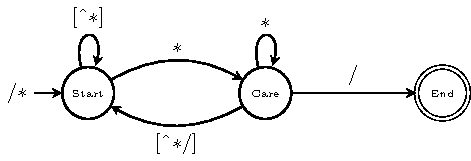
\includegraphics[width=110mm]{aut_comentarios}
\end{figure}

Usando el algoritmo visto en clase para eliminar el estado central

\begin{figure}[H]
  \centering
  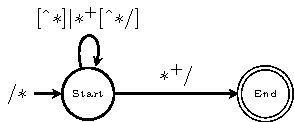
\includegraphics[width=75mm]{aut_comentarios2}
\end{figure}

Luego la expresión regular queda
/$*$([\textasciicircum $*$]$|*^+$[\textasciicircum $*$/])$^**^+$/

\subsection{Cambio en el formato de las fechas de un texto}

Mi programa detecta fechas en 5 formatos diferentes y las convierte
todas al mismo formato, que se solicita como parámetro. Los formatos
que acepta son:

\begin{itemize}
\item dd/mm/aaaa
\item dd-mm-aaaa
\item dd de $<$mes en español$>$ de aaaa
\item dd $<$mes en inglés$>$ aaaa
\item $<$mes en inglés$>$ dd, aaaa
\end{itemize}

\section{Uso}

He incluido un archivo de prueba llamado {\tt example.txt} y también
un script llamado {\tt compile\&run.sh} para lanzar el programa sobre
este fichero. Una vez ejecutado, se solicita el formato de fecha al
que convertir todas las fechas del documento en alguno de los 5
formatos reconocidos.

\end{document}